%% 
%% Copyright 2007-2020 Elsevier Ltd
%% 
%% This file is part of the 'Elsarticle Bundle'.
%% ---------------------------------------------
%% 
%% It may be distributed under the conditions of the LaTeX Project Public
%% License, either version 1.2 of this license or (at your option) any
%% later version.  The latest version of this license is in
%%    http://www.latex-project.org/lppl.txt
%% and version 1.2 or later is part of all distributions of LaTeX
%% version 1999/12/01 or later.
%% 
%% The list of all files belonging to the 'Elsarticle Bundle' is
%% given in the file `manifest.txt'.
%% 

%% Template article for Elsevier's document class `elsarticle'
%% with numbered style bibliographic references
%% SP 2008/03/01
%%
%% 
%%
%% $Id: elsarticle-template-num.tex 190 2020-11-23 11:12:32Z rishi $
%%
%%
\documentclass[preprint,12pt]{elsarticle}

%% Use the option review to obtain double line spacing
%% \documentclass[authoryear,preprint,review,12pt]{elsarticle}

%% Use the options 1p,twocolumn; 3p; 3p,twocolumn; 5p; or 5p,twocolumn
%% for a journal layout:
%% \documentclass[final,1p,times]{elsarticle}
%% \documentclass[final,1p,times,twocolumn]{elsarticle}
%% \documentclass[final,3p,times]{elsarticle}
%% \documentclass[final,3p,times,twocolumn]{elsarticle}
%% \documentclass[final,5p,times]{elsarticle}
%% \documentclass[final,5p,times,twocolumn]{elsarticle}

%% For including figures, graphicx.sty has been loaded in
%% elsarticle.cls. If you prefer to use the old commands
%% please give \usepackage{epsfig}

\usepackage{graphicx}
\usepackage[graphicx]{realboxes}
\usepackage{rotating}
\usepackage{amsmath,amssymb,amsfonts}
\usepackage{algorithmic}
\usepackage{textcomp}
%\usepackage{xcolor}
\usepackage[table,xcdraw]{xcolor}
\usepackage{hyperref}
\usepackage{url}

\usepackage{algorithmic}
\usepackage{graphicx}
\usepackage{subcaption}
\usepackage{mwe}
\usepackage{textcomp}
\usepackage{xcolor}
\usepackage{comment}
\usepackage{multirow}

\newcommand{\stefano}[1]{{\color{blue}{\textbf{[Stefano]}~#1}}}
\newcommand{\sara}[1]{{\color{red}{\textbf{[Sara]}~#1}}}
\newcommand{\gamm}[1]{{\color{green}{\textbf{[Gianlu-Matte]}~#1}}}
\newcommand{\martino}[1]{{\color{yellow}{\textbf{[Martino]}~#1}}}
\newcommand{\storyline}[1]{{\color{gray}{~#1}}}
\newcommand{\todo}[1]{{\color{cyan}{\textbf{[TODO:]}~#1}}}

\usepackage{hyperref}
\usepackage{adjustbox}
\usepackage{lineno,hyperref}  
\usepackage[margin=2.5cm]{geometry}
\usepackage{cleveref}
\modulolinenumbers[5]
\renewcommand{\baselinestretch}{1.25}


\journal{Computer Methods and Programs in Biomedicine}

\begin{document}

\begin{frontmatter}

%% Title, authors and addresses

%% use the tnoteref command within \title for footnotes;
%% use the tnotetext command for theassociated footnote;
%% use the fnref command within \author or \address for footnotes;
%% use the fntext command for theassociated footnote;
%% use the corref command within \author for corresponding author footnotes;
%% use the cortext command for theassociated footnote;
%% use the ead command for the email address,
%% and the form \ead[url] for the home page:
%% \title{Title\tnoteref{label1}}
%% \tnotetext[label1]{}
%% \author{Name\corref{cor1}\fnref{label2}}
%% \ead{email address}
%% \ead[url]{home page}
%% \fntext[label2]{}
%% \cortext[cor1]{}
%% \affiliation{organization={},
%%             addressline={},
%%             city={},
%%             postcode={},
%%             state={},
%%             country={}}
%% \fntext[label3]{}

\title{Privacy-Preserving LLM-Based Chatbots for Chronic Disease Self-management}

%% use optional labels to link authors explicitly to addresses:
%% \author[label1,label2]{}
%% \affiliation[label1]{organization={},
%%             addressline={},
%%             city={},
%%             postcode={},
%%             state={},
%%             country={}}
%%
%% \affiliation[label2]{organization={},
%%             addressline={},
%%             city={},
%%             postcode={},
%%             state={},
%%             country={}}

\author[label1]{Sara Montagna\corref{cor1}}
\ead{sara.montagna@uniurb.it} 
\ead[url]{https://www.uniurb.it/persone/sara-montagna}
\author[label1]{Sfefano Ferretti}
\author[label1]{Lorenz Cuno Klopfenstein}
\author[label1]{Michelangelo Ungolo}
\author[label3]{Martino Francesco Pengo}
\author[label2]{Gianluca Aguzzi}
\author[label2]{Matteo Magnini}

\cortext[cor1]{Corresponding author}
\affiliation[label1]{organization={Department of Pure and Applied Sciences, University of Urbino},
             addressline={Piazza della Repubblica, 13},
             city={Urbino},
             postcode={61029},
             state={Italy}
             }

\affiliation[label2]{organization={Department of Computer Science and Engineering, University of Bologna},
             addressline={Via dell'Università, 50},
             city={Cesena},
             postcode={47521},
             state={Italy}
             }

\affiliation[label3]{organization={Istituto Auxologico Italiano IRCCS \& University of Milano-Bicocca},
             addressline={Faculty of Medicine},
             city={Milan},
             %postcode={47521},
             state={Italy}
             }

\begin{abstract}
\begin{comment}
%
Medical chatbots are enabling a new way of providing medical services and are becoming a crucial component of telemedicine applications.
%
Large Language Models~(LLMs) have shown potential in improving chatbot-based systems in healthcare. However, their adoption in clinical practice faces several challenges, among which reliability issues, the need for clinical trials, and privacy concerns.

In this paper, we provide a discussion of the main issues that arise once adopting LLMs for medical chatbots in the context of chronic disease self-management, and accordingly, we define an architecture specifically devised to deal with such issues.
%
In particular, we compare two different possible solutions aimed at preventing sensitive data from being disclosed to third parties while, at the same time, offering a compelling LLM-based experience. 
%
The first one is based on the idea of having a filtering mechanism such that sensitive data is treated locally while general sentences are transmitted to an external LLM (e.g., GPT-3.5). The second approach resorts to a locally deployed LLM that exploits open-source models, eliminating the risk of data exposure. 

Experimental results underscore the challenges in effectively instructing the local LLM so as to provide performances comparable to GPT-3.5 for all the required tasks. 
%
However, among the six open models we tested, two emerges as providing highly reliable and accurate answers according to domain experts evaluation, similar or even better to those provided by GPT-3.5.
\end{comment}
\emph{Background and Objective}: 
%
Medical chatbots are reshaping the delivery of medical services and becoming integral to telemedicine, propelled by advancements in Large Language Models (LLMs). 
%
Despite their potential to enhance healthcare chatbot systems, LLMs’ integration into clinical settings is hindered by reliability concerns, the need for clinical trials, and privacy issues. 
%
This study aims to explore these challenges in the context of chronic disease self-management.

\emph{Methods}: Accordingly, the paper proposes a tailored architectural solution and a workflow that address these challenges, while preserving the benefits of LLMs.
%
We examine two solutions to prevent the disclosure of sensitive information: \emph{(i)} a filtering mechanism that processes sensitive data locally but leverage a robust online LLM (GPT-3.5 Turbo in this study) for engaging with the user effectively, and \emph{(ii)} a fully local deployment of open-source LLMs.
%
The effectiveness of these solutions is assessed in the context of hypertension management across various tasks, ranging from intent recognition to proper emphatic conversation.
%


\emph{Results}: 
The comparative analysis underscores that GPT-3.5 Turbo outperforms local models in the majority of the considered tasks. 
%
However, our examination of six open models identified two that consistently provided reliable and accurate responses to general conversations,  earning higher scores by domain experts.


\emph{Conclusions}: The study underscores the viability of incorporating LLMs into medical chatbots for chronic disease management while addressing privacy and reliability concerns.
%
Our findings suggest that carefully selected and configured Open-LLMs can offer a privacy-preserving, yet promising alternative to external LLM services, such as those of the GPT family, fostering safer and more reliable telemedicine practices.
%
Future efforts will focus on fine-tuning local models to enhance their performance across all tasks.
%
\end{abstract}



%%Graphical abstract
%\begin{graphicalabstract}
%\includegraphics{grabs}
%\end{graphicalabstract}

%%Research highlights
%\begin{highlights}
%\item Research highlight 1
%\item Research highlight 2
%\end{highlights}

\begin{keyword}
Large Language Model \sep Medical Chatbot \sep Chronic Disease Self-Management \sep Patient Empowerment
\end{keyword}

\end{frontmatter}

%% \linenumbers

\section{Introduction}

Recent advancements in generative AI have opened the door for using powerful deep learning techniques that could be used in health-related contexts and potentially support health information-seeking.
%
However, when asking ChatGPT~(GPT-4) ``\emph{which are the main issues in applying LLMs for building a chatbot supporting chronic patients?}'' this is one answer you can get (in 50~words):
%
\begin{quote}
The main issues in using Large Language Models~(LLMs) for chronic patient support chatbots include accuracy in medical information, maintaining patient privacy, handling nuanced patient emotions, ensuring context-specific advice, and managing the limitations in understanding complex medical conditions or treatment details.
\end{quote}
%
Even though there is a huge discussion around the application of LLMs in medicine, their application in the clinical context, especially for home-care, is far from being resolved.
%
In fact, despite the capabilities and the widespread diffusion of LLMs, their exploitation in the context of patient self-management still poses a number of issues that are worth to be discussed and explored for this approach to support the clinical practice.
%
For instance, in addition to the risks of generating unfaithful or factually incorrect outputs, it is fundamental to establish mechanisms that prevent the transmission of sensitive medical data to external LLM systems, ensuring robust privacy safeguards in healthcare chatbot applications. 
%
This need comes not only from common sense, but also from the need to adhere to laws and regulations, such as the Health Insurance Portability and Accountability Act~(HIPAA)~\cite{hipaa}, or General Data Protection Regulation~(GDPR)~\cite{gdpr,Zichichi20224515}.

In this paper, we present the data workflow of an LLM-based chatbot designed for patient self-management.
%
The workflow is designed to provide data security and to preserve the high performance of LLMs.
%
The system comprises different components: a back-end for data storage and analysis and a front-end service for user-interaction, which is based on user query processing through Natural Language Processing~(NLP) and answer generation via Natural Language Generation~(NLG).
%
The most critical part, the NLP\&NLG module, is devised for managing patient queries by handling the above-mentioned privacy and security issues, as well as reducing the risk of misinformation by confining the conversation to sentences strictly related to general information on the specific disease the chatbot is designed for.
  
For this purpose, we devised and tested two alternative solutions.
%
%The aim of the two alternative strategies is to ensure the quality of the chatbot responses while being constrained based on the identified requirements.
%
% They both rely on a sequential approach based on two modules that work in a pipeline. 
%
The first solution aims at leveraging the full potential of online reference LLM services.
%
It is composed by two modules.
%
The first one takes the input by patients and extracts the intent of the question. 
%
A machine learning pipeline, implemented using ML.NET 2.0\footnote{\url{https://learn.microsoft.com/en-us/dotnet/machine-learning/}}, is trained to recognise the user's intent and classify the input according to whether it contains sensitive data or not. 
%
If the input contains sensitive data, it is handled locally using classical methods to parse strings and extract data. 
%
If the input does not, it is forwarded to a third-party LLM (GPT-3.5 Turbo in the paper)  through an API call, with a properly fine-tuned prompt, in order to obtain a compelling answer \cite{MontagnaGoodIT2023}.
%
% The two strategies differ in the technologies behind the two modules. 
%In particular, we exploited a machine learning pipeline implemented using ML.NET 2.0\footnote{\url{https://learn.microsoft.com/en-us/dotnet/machine-learning/}} to recognise the user's intent.
%
%Some intents can be handled right away through a hard-coded pathway, delivering immediate response to the user.
%
%Requests that are classified as not containing sensitive data are forwarded to a third-party LLM (e.g., GTP-3.5) through an API call, thus generating the reply.
%
%In our previous work \cite{MontagnaGoodIT2023},  we proposed a preliminary overview of a system using this kind of strategy.
%
%However, we did not perform any comparison with other strategies, nor did we evaluate the accuracy of the classification of intents.
% Furthermore, after that initial proposal, the software architecture was improved by switching from the use of the external WIT.ai service to a more reliable and local intent detection model based on ML.NET.

The second solution is based on the idea of having a local open-source LLM (like Llama2~\cite{llama2} or Mistral~\cite{mistral}) served through its HTTP API (like fastchat~\cite{fastchat} or ollama\footnote{\url{https://github.com/jmorganca/ollama}}).
%
This approach completely avoids sensitive data disclosure, since the model is running locally on-premises, but requires complex system instruction via ad-hoc prompts, Retrieval Augmented Generation~(RAG)~\cite{rag} approaches, or model fine-tuning.
%
Six open-source LLMs have been evaluated in this paper.

We performed an evaluation of the two approaches using a dataset of simulated patient queries. 
%
Experimental evaluations is performed across various tasks, encompassing intent recognition, parameter extraction and general conversation. 
%
The performances are compared according to well-established metrics and conducting a comprehensive evaluation by domain experts.
%
Our preliminary results show how the first approach performs better than the second one in terms of intent recognition and parameter extraction. 
%
However, there are two major shortcomings of the first approach, that are: 
%
\emph{(i)}~the risk that some sensitive data can be passed on to the third-party LLM system, either due to errors in the classification module or due to the ambiguity of the input and
%
\emph{(ii)}~the cost associated with third-party technologies, which affects how democratic the solution is.
%
Moreover, in this paper, we identified two Open-LLMs, Alfred and Mixtral~\cite{mixtral}, whose responses received higher scores by domain experts.
%
This indicates their potential as promising candidates for further refinement and enhancement in specific tasks through tailored fine-tuning efforts.

%this system is probably less effective (in terms of answer generation) when sentences with sensitive data are submitted, since no LLM is used in this case and ii) . 
% + è a pagamento e proprietario di azienda esterna - non abbiamo alcuna certezza che il servizio continuerà ad essere disponibile ecc...
%More detailed experiments are needed to better instruct the local LLM solution and to improve the robustness and accuracy of the classification module.
%%% SF ADD


% Alcuni punti:
% - removing Wit.AI (no more supported) and replacing with...
% - managing with an opportune prompt engineering the type of answers the LLM can provide
% - comparing the performance of the adoption of a pure LLM ...

% discussing pro and cons

% Il contributo è soprattutto capire se gli OPEN-LLM ci supporterebbero e cosa questo comporta.

In summary, the paper contributes to the advancement of LLMs in healthcare by proposing a robust workflow and evaluating alternative strategies tailored specifically for patient self-management within the clinical care context.
%
The emphasis on privacy, security, and accuracy underscores the significance of these advancements in improving healthcare delivery.
%
With respect to our previous findings~\cite{MontagnaTELMED2024}, where the first strategy seemed to have no competitors, further evaluations with additional methods and the exploration of novel emerging open-source models, present fresh prospects for the adoption of open models within this domain. 
%
%Future work will be devoted to 



\section{Background}\label{sec:back}

LLMs hold the premise for a deep revolution in medicine. 
%
Among the others, ChatGPT, which is based on the Generative Pretrained Tranformers (GPT family), deserved to jump to the headlines given its impressive ability to understand human language and to produce human-like conversations.
%
Many alternatives exist, and the list of pretrained models is continuously growing and updated.
%
They differ in model accessibility -- open (e.g., Mistral), licensed (e.g., Llama2), closed (e.g., GPT-X) --, languages supported --multilingual or subset of few specific languages --, architecture-- encoder-decoder, casual decoder, prefix decoder.
%
Some works have been already done towards medical-domain specific LLMs, such as Google Med-PALM2.

\subsection{LLM-based Chatbot}

%%% Narrazione:
The adoption of chatbots in the context of medicine, as a tool to support patient needs and caregivers in their work, is already well known in literature \cite{3419368}. 
%
For instance, conversational agents are a well known approach to implement personal cognitive assistants \cite{Sulis2023}.
%
However, since the advent of LLMs, the interest of the scientific community is incredibly increased and the discussion around this theme is impressively lively \cite{Thirunavukarasu2023,Clusmann2023,Tian2023,cascella2024}.
% 
Main experiences in the adoption of LLM-based chatbots in medicine, without claiming to be exhaustive, are devoted to:
%
\begin{enumerate}
    \item There is a general agreement that LLM-based chatbots may become a methodological tool assisting physicians or nurses, during their clinical practice, in various areas of medicine. 
    %
    As an example, they may support clinical decisions, by abstracting key results from literature. Or they can detect medical errors, by identifying discrepancies between diagnosis and treatment.

    \item On the patient side, they may be a crucial component for bootstrapping patient empowerment by providing trustworthy and emphatic answers to user queries. In this context, they must resemble a dialogue between the physician and the patient which is a key element to provide an effective and compassionate care. Moreover, they should be able to proactively suggest actions, reasoning on tracked patient activities and vital signs dynamic.

    \item In research, an LLM-based chatbot may assist basic research by automating certain tasks, such as data analysis, acquisition and interpretation, summarising information, paraphrasing text, scientific literature search for medical knowledge and related work extraction.

    \item In medical education, an LLM-based chatbot may be used to provide teaching material and as a tool for students who can benefit from interacting tutoring. In this context, noteworthy are the very good performances demonstrated in passing medical examinations. 

\end{enumerate}
%
\noindent In particular, it should be clarified that incorporating and integrating an LLM in a new application that exploits its NLP/NLG abilities poses a higher level of complexity in modelling, designing and implementing the whole system, than querying an LLM-based chatbot via a web interface.
%
Indeed, even though literature reports an increasing number of work in these areas, a realistic vision in this context foresees extensive validation and further development to overcome a set of issues that literature clearly highlights  \cite{Wang2023,Mesko2023}:
%
\begin{itemize}
    \item Ethical concerns, including risks of privacy and security \cite{lancet2023}: third-party technology, such as ChatGPT, carries an inherent risk of compromising patient privacy, if patients enter test results, photos of their face, communication information, and more. All of this vital health information is collected and stored, potentially compromising patient privacy. 
    %
    Open-LLMs, locally deployed, seem the most obvious choice to handle these concerns.
    %
    Although the performances shown against benchmarks are impressive, further domain-specific evaluation is required to demonstrate their effectiveness in medicine, and ad-hoc fine-tuning to deal with inaccuracy, uncertainty and misinformation; this is true for each of the applications listed above, but especially if chatbots are meant to interact with patients without the intervention of a domain expert.
     
    \item Proposed integrated solutions have to take into account economic costs, hardware requirements and environmental impact in order to develop a democratic and sustainable technology.
    
\end{itemize}
%
In these respects, the results reported so far strongly encourage further research and evaluation. 
%
However, to the best of our knowledge, there are still no work assessing the applicability and performance of LLMs in the context of the hypertension chronic disease self-management.
%%%%

\section{Methods}



\subsection{Architecture}\label{subsec:archi}

In this paper we focus on %the identification of 
an architecture to support patient empowerment by exploiting an LLM-based chatbot designed to fit patient needs in the context of chronic diseases.
%
The system architecture is meant to fulfil two main requirements: 
%
i) the system must support the acquisition of patient data, while ensuring privacy and security, and 
(ii) must provide trustworthy answers to a limited set of in-topic queries.
%
The system's architecture is depicted in Figure~\ref{fig:arch}. 
 It encompasses four main components: a Chatbot, an NLP\&NLG module for understanding user inputs and reacting properly, a Database to store data and 
 a Data Processing Unit to provide some kind of data elaboration, for instance by statistic functions or data visualisation.
%
In the following, we describe the requirements to be satisfied by each component, as well as how they interact.

% Da valutare se mettere la figura in doppia colonna o colonna singola.
% Se la caption rimane così lunga forse meglio che occupi tutte e due le colonne.

\begin{figure*}[t]
	\centering
	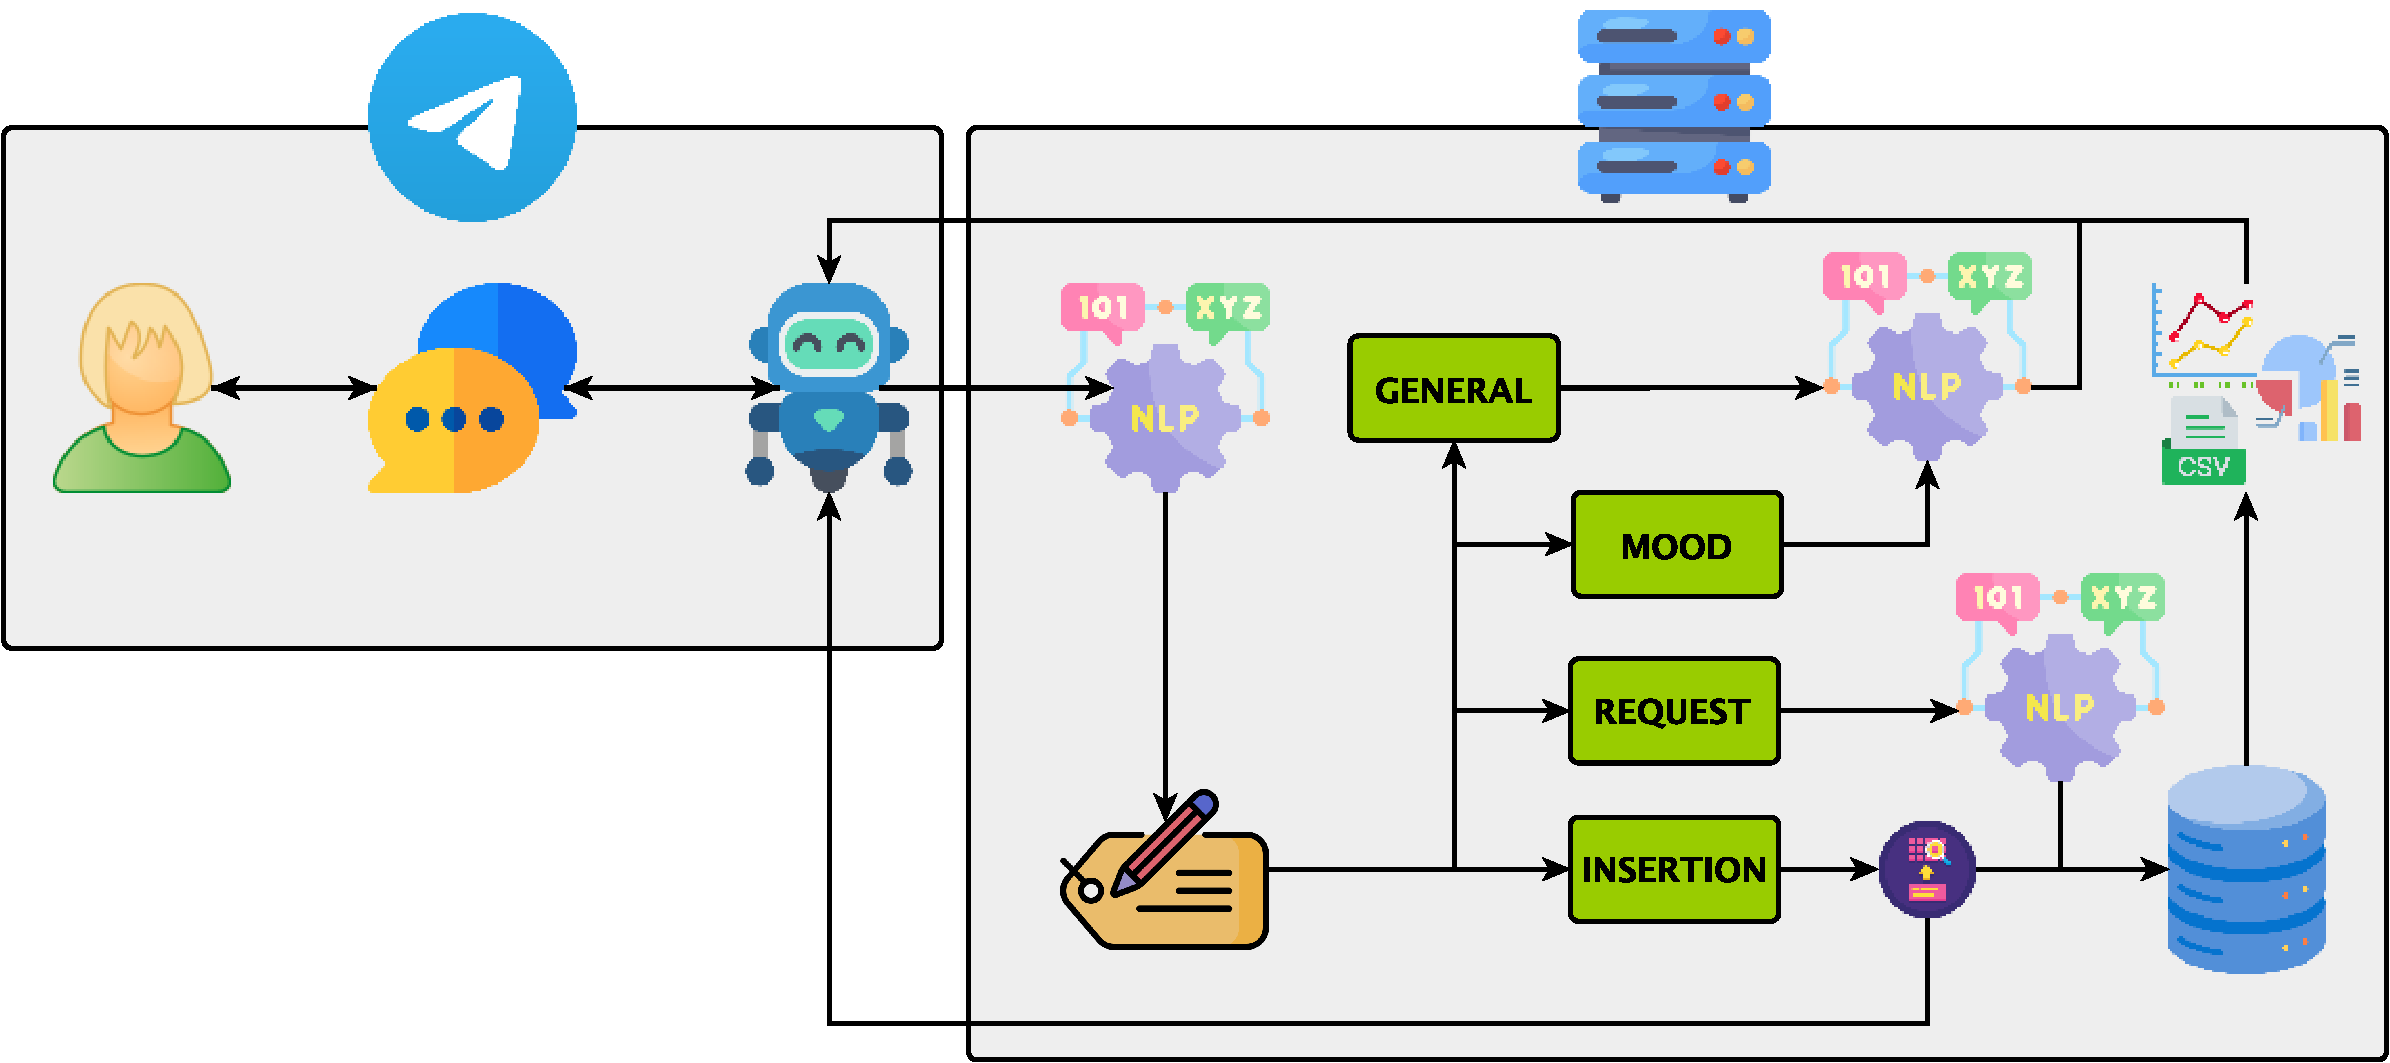
\includegraphics[width=0.8\textwidth]{figures/system_scheme_3llm.pdf}
	\caption{
            System architecture.
            %
            The patient interacts with the chatbot through an instant messaging application.
            %
            Upon receiving a message, the chatbot forwards it to a server. 
            %
            The message is then categorised by an LLM into one of four categories: mood, request, insertion, or general---see \ref{subsubsec-nlp} for more details. 
            %
            %Mood indicates the patient is expressing personal feelings about their health. 
            %
            %Request signifies the patient's need for specific information. 
            %
            %Insertion involves the patient sharing their health measurements or other relevant data.
            %
            %For messages that don't fit these categories, they are labelled as General. 
            %
            %This includes inquiries about hypertension (e.g., how to measure blood pressure) and other topics unrelated to the immediate context. 
            %
            General and mood messages are immediately propagated to an LLM to generate the response.
            %
            Insertion and request messages are post-processed by a parsing and LLM phase respectively to identify the parameters for the query to perform on the DB.
            %
            After that, an acknowledgement message is sent to the user in the scenario of insertion.
            %
            Instead, in the case of a request, the response is generated from the extracted data in the format specified by the user (e.g., graph, list, etc.).
        }
	\label{fig:arch}
\end{figure*}


% qui descrivere bene i componenti e che ruolo ci si aspetta abbiano, nonché il flusso dell'informazione: Cosa mi aspetto da ciascun componente
\subsubsection{Chatbot}

The chatbot is the component in charge of the interaction with patients and, as such, it must be designed for interacting with users whose digital skills are the most varied. Accordingly, it must be multiplatform, and easy to install and use.
%
Moreover, to motivate and engage patients, particular attention should be given to the user experience, through a suitable and effective user interface.

\subsubsection{Database}
Patient data needs to be stored in order to allow for proper medical monitoring and diagnosis. 
Also, discussions, or some historical records of discussions made, might be important to improve the quality of the interactions with the user over time. 
Possible solutions range from a local database, which is the classic and straightforward solution to properly manage data in a client-server approach, to those already presented in our previous works \cite{MontagnaGoodIT2023} leveraging distributed solutions which take into account also for data sovereignty requirements.

\subsubsection{NLP\&NLG}\label{subsubsec-nlp}

The component in charge of understanding the human language and generating answers with a human-like language is the most critical one.
%
We expect patient to input almost every kind of sentence, which can span from general questions, regarding every aspect of their life, to specific questions related to their disease. 
%
Disease-related questions can vary from input data, request statistics and/or general information on their physical health state.

In this respect, there are several issues to deal with:
\begin{enumerate}
    \item if NLP\&NLG is provided on top of LLMs owned by private companies, data privacy and security are not granted: inputs containing sensitive data must be intercepted and managed accordingly;
    \item the chatbot is typically devised for a specific medical domain. As such, it must not provide answers to every question the patient may input, but kindly remind the user of the tasks it is in charge of;
    \item answers must be precise and emphatic, to improve user experience and trust, crucial elements for patient engagement and self-management;
    \item the context of the prompt should be precisely fine-tuned in a way that answers are limited to the medical task at hand and no misinformation are produced.
\end{enumerate}
%
\noindent With these requirements in mind, we identified four categories for the patient inputs, which represent the intents associated to each question. At each category, the execution of a different flow is associated.
%
\begin{description}  
    \item[\textbf{Insertion}] The first category includes all the sentences that contain sensitive data, which can be vital signs, as well as general personal information, such as anthropometric measurements, anamnestic data, lifestyle, demographic information, medical histories. 
    %
    Such information can not be prompted to a third-party LLM but, since the interpretation must be reliable, an ad-hoc parser must be developed to extract relevant data from the sentence.
    %
    \item[\textbf{Request}] This category encompasses all the inputs specifically requesting to inspect patient data. 
    This request does not typically contain sensitive information and an LLM may support the identification of the request parameters, 
    such as which data the patient wants to inspect, since when and in which format. For instance, in response to the query: \emph{Please provide me with a plot of the last week's values of my blood pressure}, the LLM must extract: \texttt{PRESSURE 7 GRAPH}. These parameters are used to opportunely invoke the data processing unit.
    %
    \item[\textbf{Mood}] Sentences referring to how the patient feels about their pathology must be specifically addressed by leveraging stored data analysis to inform patients about their condition, and possibly encourage and comfort them.
    %
    \item[\textbf{General}] It includes all the other questions. They can be managed by an external an LLM-service via proper prompts: if they are out of scope, the chatbot will remind its tasks and will suggest to ask proper experts for an answer. 
\end{description}

%\sara{deve emergere bene il fatto che peraltro il nostro chatbot non deve rispondere a tutto, perché così gestiamo anche il problema dell'accuratezza e della misinformazione--deve rispondere al minimo indispensabile per essere carino e incoraggiante...}

%% raggruppiamo in tre categorie:
% inserimento
% lettura (restituisce il numero di giorni antecedenti la data odierna da cui calcolare media ecc oppure fare il grafico)
% generale



\subsubsection{Data processing}

%grafici, valori medi, lista valori
The data processing unit is in charge of conducting a different set of computations over the data stored for each patient.
%
It specifically responds to the requests identified by the NLP module (under the \emph{request} category) by providing -- over the period of time specified within the request by the user -- the curve diagram of the blood pressure, or the mean or the list of all the stored values.

\vspace{5pt}
\noindent The sequence diagram describing the flow of data through these components is reported and described in Figure~\ref{fig:seq}.

%%%%
%come mi aspetto che funzioni l'interazione tra il chatbot e il sistema dietro???
\begin{figure}[ht!]
	\centering
        % ////www.plantuml.com/plantuml/png/fPB1QiCm44Jl-nLgJiuXFs1e2I6NGdeg_G1XJrDJMKftrw7z-ofrBHGB6feSRF3CChlpy5hKiWwzepjzGmzpSBRpH2y2Dgi7imbQ6u5lgrxsIugV9_KPV0JdngYOLJGNZrxXrMoXQ3JmeZQDioBTwzSuQnljZbPHJbAXcDLytK_Mabhy4KFMwRZKt9lE2rXfEZ7BErWMp6uQlHIVbBpXTbF_fbQjLPlQd_6opNlYTQAPomGdI0SoFWQ8KhvYjtkg9sDsORGeFcTa6788Nb35IhPFUDBysV4fE4rFiz6axQPaFhPiaS-LE1j6z2g6X84R_0Dg-QFbu98y1zU7q9RKJkfbP2dq4gicUCMdLeE0ho9rOyazFDWwAefEpWrThpZDjxIEhw5ttm00
	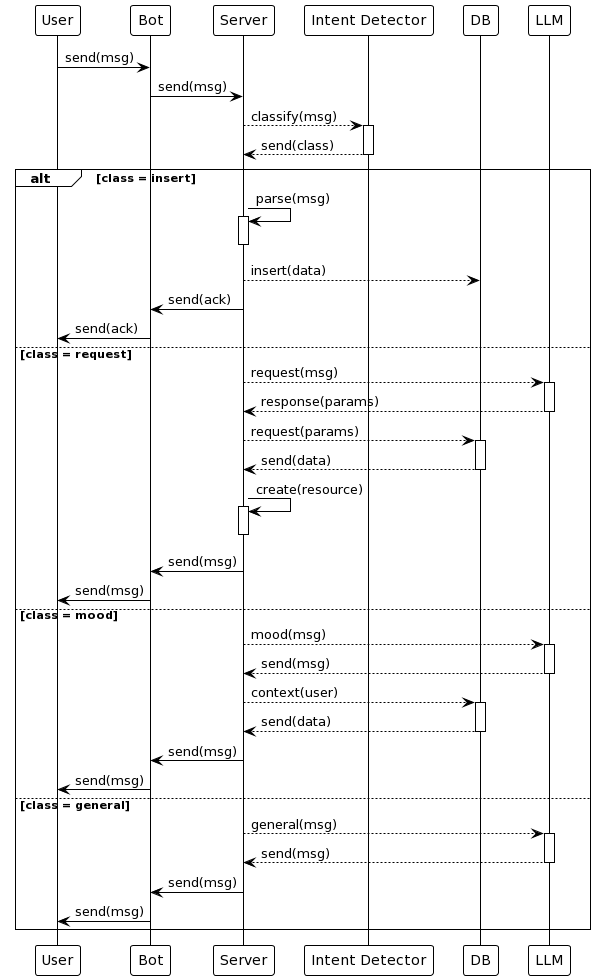
\includegraphics[width=0.6\textwidth]{figures/sequence_diagram.png}
	\caption{
            Sequence diagram of the interaction between the patient and the chatbot. 
            Initially, the patient starts the communication by sending a message. 
            First, the chatbot sends it to the server that classifies it. 
            If the message is a request for inserting new data, then the message is parsed to retrieve the information. 
            At this point, the system writes the new data on the DB and replies to the patient with an acknowledgement message. 
            If the user is requesting data stored by the system, then the message is further analysed by an LLM that extracts the parameters for the query on the DB.
            Finally, if the message concerns the patient’s mood or it is a general request (possibly also out of context) then the LLM generates a free text response for the patient.
        }
	\label{fig:seq}
\end{figure}
%%%%
\subsection{Prototype}\label{subsec:proto}

The prototype we are presenting here is specifically devised for hypertensive patients.
%%% SPECIFIC CONTEXT
\subsubsection{Chatbot for Hypertensive Patients}

The adoption of chatbots in cardiovascular medicine holds immense potential, particularly in the context of cardiovascular prevention. 
%
Leveraging LLM-based chatbots can revolutionise patient care by providing timely, personalised, and evidence-based information. 
%
Regarding hypertension management, chatbots can play a pivotal role in patient education, medication adherence and lifestyle modification guidance. 
%
They can also improve the quality of blood pressure measurement in the domiciliary setting which is often suboptimal according to a recent survey \cite{Mancusi2022}.
%
These chatbots, equipped with the ability to comprehend natural language, can engage in meaningful conversations with patients, offering real-time support and answering simple queries. 
%
Even though they cannot substitute healthcare professionals, they can facilitate remote patient monitoring, enabling healthcare providers to track vital signs and adjust treatment plans as necessary. 
%
The efficiency of chatbots in collecting patient data and providing continuous support needs proper validation in observational studies but can potentially and significantly enhance the overall quality of care, making them a valuable tool for physicians seeking to optimise cardiovascular health outcomes. 
%
By integrating chatbots into the healthcare system, we can foster a more proactive and preventive approach to cardiovascular medicine, ultimately improving patient outcomes and reducing the burden on healthcare resources.

\subsubsection{Prototype implementation}
%
%\stefano{please expand on practical challenges and real-world implementation nuances might enhance its practical relevance.}
The prototype is set up as a Telegram chatbot that interacts with its users through a conversation within the messaging service's mobile app.
%
The chatbot is implemented as a .NET~Core Web service and a MongoDB database for data storage.
Both components run on-premises on a dedicated server in order to grant data security and isolation.

%%% SF add:
The decisions we made enabled us to establish a practical prototype system to evaluate the feasibility of using LLM-based chatbots for chronic disease self-management. However, implementing this system in a real-world scenario presents several challenges.
For example, while utilising local dedicated servers provides complete control over data and processing, it also necessitates resource allocation and ongoing maintenance. Furthermore, practical considerations such as scalability, backup and recovery procedures, and potential hardware failures must be addressed. These issues could potentially be mitigated by transitioning to a cloud-based service.
%%%%

Basic chatbot functionality is implemented in the fashion of a simple state machine, handling basic conversation turns, while most requests are handled by a specific NLP\&NLG module.
%%% SF add:
The state machine enables us to control the conversation flow, understand the user’s intentions, and handle sensitive data securely without disclosing it to third-party software. However, this approach can limit the interaction’s flexibility and naturalness due to its reliance on predefined rules and responses. To enhance the level of naturalness where possible, we employ a separate module dedicated to natural language processing and generation.

In this paper, we devise and compare two possible solutions for the architectural model presented in the previous section.
%
Both solutions are specifically meant to prevent sensitive data from being shared with third-party services.
%
In particular, we propose two solutions: \emph{i} a solution that is grounded on two components, the first one trained to detect sentences with personal information, the second one that exploits GPT-3.5 Turbo to respond to those inputs that are not classified as potentially sensitive, and \emph{ii} a solution based on open-source LLMs which are locally installed, 
so that personal data are not shared once processing user inputs.
%%% SF add:
The first solution proposes a hybrid approach, integrating a custom classifier with a state-of-the-art LLM, to strike a balance between privacy and performance. However, this approach requires reliance on a third-party service, which could introduce some risks and limitations.
%
The second solution operates under the assumption that open-source LLMs can deliver a satisfactory level of performance and quality for our chatbot, without compromising the user’s privacy. However, exploiting Open-LLMs comes with a price, since downloading and installing and exploiting large models can be both costly and time-consuming. Additionally, these models may require fine-tuning to the specific domain and task, if they do not demonstrate good performances.
%

The goal of this work is to compare and evaluate the feasibility of both solutions. The results of this comparison will be presented in Section \ref{sec:eval}.

\subsubsection{ML.NET~2.0 and GPT-3.5 Turbo}
%\gamm{guardare codice Mic}
%\stefano{qui avevamo detto che potevamo mettere qualche dettaglio in più guardando il pezzo di codice scritto da Michelangelo per invocare le funzioni della libreria}
This solution exploits the ML.NET~2.0\footnote{\url{https://learn.microsoft.com/en-us/dotnet/machine-learning/}} library, developed for C\# application, to classify textual data and perform sentiment analysis to recognise user intent. 
%
%ML.NET~2.0 adopts NAS-BERT to compress large BERT transformers \cite{nas-bert}.
%
As such, text classification can be performed through a variety of compressed models that do not suffer from big computational and memory costs.
In particular, the developed code defines a ML pipeline that includes various data transformations and a multiclass classification trainer. 
%
The ML.NET~2.0 framework grounds on a pipeline that includes steps to feature text, concatenate and normalise features, and finally apply a one-versus-all multiclass classification thanks to a logistic regression binary estimator. This is the specific pipeline used:
\begin{itemize}
    \item \emph{FeaturiseText}: which transforms a text column into a featured vector that represents normalised counts of n-grams, this is essential to use the words as input to our regression model;
    \item \emph{Concatenate}: which concatenates the obtained values into a single one;
    %\item \emph{Map Value to Key:}  %% ha senso saltarla
    \item \emph{Normalise}: which scales the features to a range between 0 and 1.
    \item \emph{One Versus All Multiclass Classification}: that trains a set of binary classifiers, one for each class. Each predictor is trained to distinguish one class from all other classes. It uses L-BFGS logistic regression as the binary classifier.
    %\item Map Key to Value: %%SF  saltata anche questa    
\end{itemize}
%
The 80\% of a set that simulates a variety of possible patient queries -- defined by domain experts -- is adopted for training a Logistic Regression model with the One Versus All strategy.
%
Each sentence is labelled with one of the four intents defined above.

Downstream the first classification module, those sentences that are not classified as containing sensitive data, are passed to GPT-3.5 Turbo with different prompts: 
\begin{itemize}
    \item Request: the prompt instructs the LLM to extract the parameters from the request.
    \item Mood: the LLM is instructed to generate short text, possibly reassuring the user or suggesting to redirect their queries to a medical expert.
    \item General: the LLM is instructed to limit the response only to the clinical condition it is devised for, reminding the user the tasks of the chatbot, giving the minimal safe set of medical information, in requests are pertinent (e.g. how can I measure my pressure? results in: \quote{To measure your blood pressure, sit calmly for 5 minutes. Place the cuff on your upper arm, aligning it with your heart. Press start on the monitor. The cuff inflates, measuring systolic and diastolic pressures. Record the values, noting any unusual readings. Consult a healthcare professional for interpretation and guidance.} 
\end{itemize}

\subsubsection{Open-LLMs}
In this prototype, we utilise the REST API service named Ollama, capable of hosting various LLMs.
%
These range from smaller, like Mistral, to larger foundational models like Llama2 70 billion.
%
Our choice of this service was influenced by its API, which aligns well with the GPT family, specifically liteLLM\footnote{https://github.com/BerriAI/litellm}. This ensures a seamless transition between the two solutions without necessitating any changes to our current codebase.
%
We specifically assess the performance of Alfred, Llama2 (70, 13 and 7 billion), Mistral and Mixtral.
%
This selection is driven by our goal to match the original GPT-3.5 Turbo performance while ensuring the application remains responsive. 
%
In particular, we focus on a smaller model that can load and respond swiftly.

Our primary methodology for instructing these LLMs to execute our specified tasks relies heavily on \emph{prompt engineering}. 
%
This technique involves creating \emph{system prompts} (i.e., specifically, texts that are integrated into each query within the chat session) designed to generate specific text outputs.
%
We developed specialised prompts for each function, such as sentence classification and response generation.
%
These prompts are then refined using GPT-4, in line with the advancements in recent GPT solutions.
%
To implement the architecture outlined in the \ref{fig:arch}, we needed to utilise three distinct prompts, specifically:
\begin{itemize}
    \item Sentiment analysis prompt: This text is used to categorise a sentence based on the described content.
    \item Request handling prompt: After selecting the request, there is a second phase where it is necessary to determine the type of request made, particularly by selecting the time range, the requested data (i.e., blood pressure or heartbeat), and the format (i.e., list, average graph). 
    To achieve this, we created three prompts used in parallel to extract the required information.
    \item Response to mood and general inquiries prompt: Here, the language model should act as if it were a doctor, 
    responding in a concise yet clear and reassuring manner. We also tried to configure the bot to respond in this way.
\end{itemize}
Given these prompts, the maximum number of requests per message is four, as a) one is to understand the category and b) in cases where the category is a request, there is a scope for an additional three calls to the model.
However, since the responses are typically very short (a word), the collective performance does not suffer.
Even the largest model on a server machine can produce two words per second, even when run on a CPU.


%screenshot del bot con inserimento dati e visualizzazione valori
%--> poca roba perché il fuoco rimane sul confronto tra le due architetture

%%%%
%%%%
\section{Results}\label{sec:eval}


%!TeX root = ../paper-2024-cmpb-llm-chatbot-biomed.tex
\begin{figure}[!ht]
    \ContinuedFloat
    \centering
    \begin{subfigure}[b]{0.49\textwidth}
        \centering
        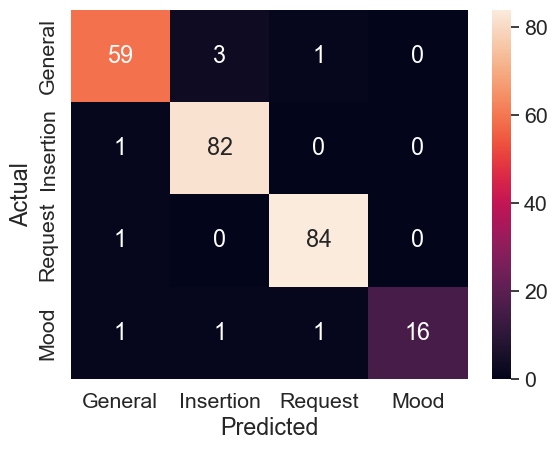
\includegraphics[width=\textwidth]{figures/confusion_matrices/nas_bert.png}
        \caption{ML.NET~2.0 framework}
        \label{fig:cm-nas-bert}
    \end{subfigure}
    \hfill
    \begin{subfigure}[b]{0.49\textwidth}  
        \centering 
        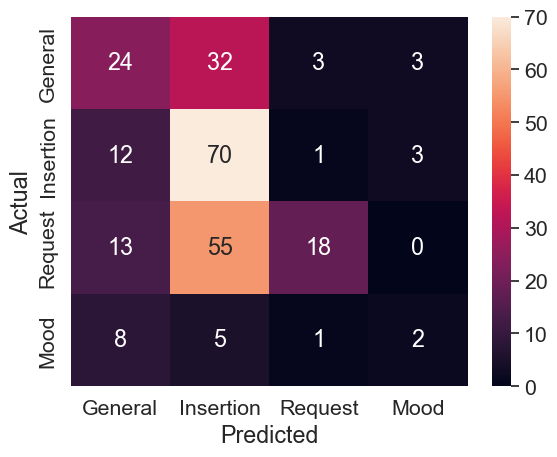
\includegraphics[width=\textwidth]{figures/confusion_matrices/alfred.png}
        \caption{Alfred}
        \label{fig:cm-alfred}
    \end{subfigure}
    \vskip\baselineskip
    \begin{subfigure}[b]{0.49\textwidth}  
        \centering 
        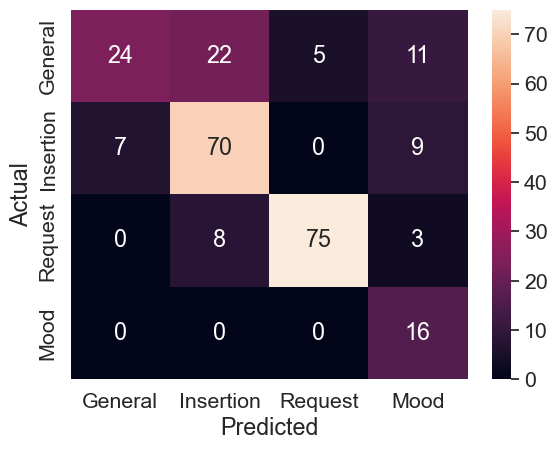
\includegraphics[width=\textwidth]{figures/confusion_matrices/llama2_70b.png}
        \caption{Llama2 70b}
        \label{fig:cm-llama70}
    \end{subfigure}
    \hfill
    \begin{subfigure}[b]{0.49\textwidth}   
        \centering 
        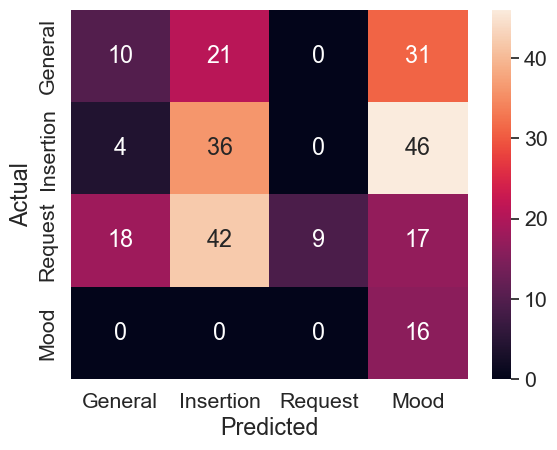
\includegraphics[width=\textwidth]{figures/confusion_matrices/llama2_13b.png}
        \caption{Llama2 13b}
        \label{fig:cm-llama13}
    \end{subfigure}
    \caption{Confusion matrices for the classification phase.}
    \label{fig:cm1}
\end{figure}
\begin{figure}[!ht]
    \ContinuedFloat
    \centering
    \begin{subfigure}[b]{0.49\textwidth}   
        \centering 
        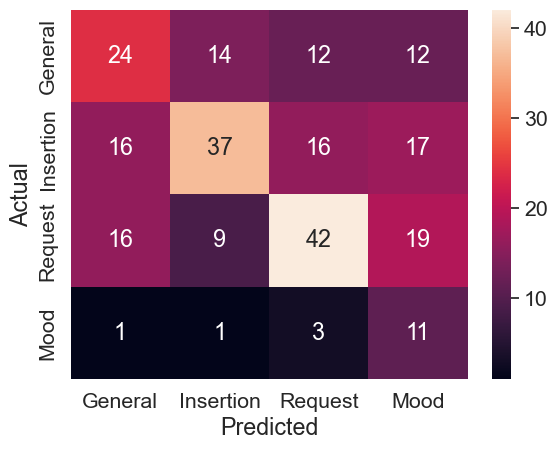
\includegraphics[width=\textwidth]{figures/confusion_matrices/llama2_7b.png}
        \caption{Llama2 7b}
        \label{fig:cm-llama7}
    \end{subfigure}
    \hfill
    \begin{subfigure}[b]{0.49\textwidth}   
        \centering 
        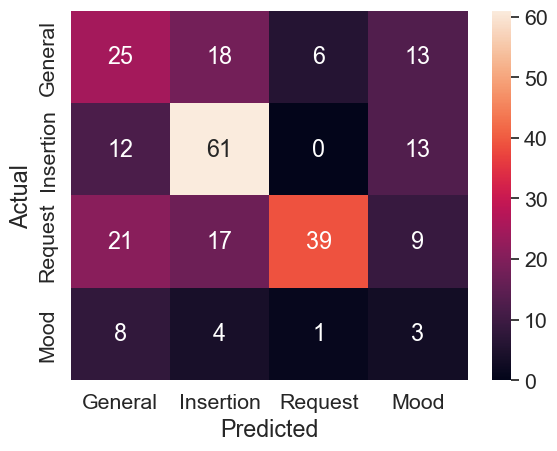
\includegraphics[width=\textwidth]{figures/confusion_matrices/mistral.png}
        \caption{Mistral}
        \label{fig:cm-mistral}
    \end{subfigure}
    \vskip\baselineskip
    \begin{subfigure}[b]{0.49\textwidth}   
        \centering 
        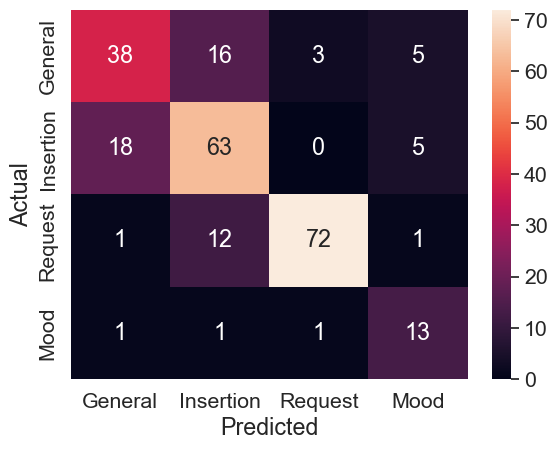
\includegraphics[width=\textwidth]{figures/confusion_matrices/mixtral.png}
        \caption{Mixtral}
        \label{fig:cm-mixtral}
    \end{subfigure}
    \caption{Confusion matrices for the classification phase.}
    \label{fig:cm2}
\end{figure}

%!TeX root = paper-2024-cmpb-llm-chatbot-biomed.tex
% Please add the following required packages to your document preamble:
% \usepackage{multirow}
\begin{table*}[]
\centering
\resizebox{\textwidth}{!}{
\begin{tabular}{|l|rrrr|rrrr|r|}
\hline
\multicolumn{1}{|c|}{\multirow{2}{*}{Model}} & \multicolumn{4}{c|}{Precision} & \multicolumn{4}{c|}{Recall} & \multicolumn{1}{l|}{\multirow{2}{*}{Accuracy}} \\ \cline{2-9}
\multicolumn{1}{|c|}{} & \multicolumn{1}{l|}{General} & \multicolumn{1}{l|}{Insertion} & \multicolumn{1}{l|}{Request} & \multicolumn{1}{l|}{Mood} & \multicolumn{1}{l|}{General} & \multicolumn{1}{l|}{Insertion} & \multicolumn{1}{l|}{Request} & \multicolumn{1}{l|}{Mood} & \multicolumn{1}{l|}{} \\ \hline
\rowcolor[HTML]{EFEFEF}
Alfred & \multicolumn{1}{r|}{0.39} & \multicolumn{1}{r|}{0.81} & \multicolumn{1}{r|}{0.21} & \multicolumn{1}{r|}{0.12} & \multicolumn{1}{r|}{0.42} & \multicolumn{1}{r|}{0.43} & \multicolumn{1}{r|}{0.78} & \multicolumn{1}{r|}{0.25} & 0.46 \\ \hline
Llama2:70b & \multicolumn{1}{r|}{0.39} & \multicolumn{1}{r|}{0.81} & \multicolumn{1}{r|}{0.87} & \multicolumn{1}{r|}{1.00} & \multicolumn{1}{r|}{0.77} & \multicolumn{1}{r|}{0.70} & \multicolumn{1}{r|}{0.94} & \multicolumn{1}{r|}{0.41} & 0.74 \\ \hline
\rowcolor[HTML]{EFEFEF}
Llama2:13b & \multicolumn{1}{r|}{0.16} & \multicolumn{1}{r|}{0.42} & \multicolumn{1}{r|}{0.10} & \multicolumn{1}{r|}{1.00} & \multicolumn{1}{r|}{0.31} & \multicolumn{1}{r|}{0.36} & \multicolumn{1}{r|}{1.00} & \multicolumn{1}{r|}{0.15} & 0.28 \\ \hline
Llama2:7b & \multicolumn{1}{r|}{0.39} & \multicolumn{1}{r|}{0.43} & \multicolumn{1}{r|}{0.49} & \multicolumn{1}{r|}{0.69} & \multicolumn{1}{r|}{0.42} & \multicolumn{1}{r|}{0.61} & \multicolumn{1}{r|}{0.58} & \multicolumn{1}{r|}{0.19} & 0.46 \\ \hline
\rowcolor[HTML]{EFEFEF}
Mistral & \multicolumn{1}{r|}{0.40} & \multicolumn{1}{r|}{0.71} & \multicolumn{1}{r|}{0.45} & \multicolumn{1}{r|}{0.19} & \multicolumn{1}{r|}{0.38} & \multicolumn{1}{r|}{0.61} & \multicolumn{1}{r|}{0.85} & \multicolumn{1}{r|}{0.08} & 0.51 \\ \hline
Mixtral & \multicolumn{1}{r|}{0.61} & \multicolumn{1}{r|}{0.73} & \multicolumn{1}{r|}{0.84} & \multicolumn{1}{r|}{0.81} & \multicolumn{1}{r|}{0.66} & \multicolumn{1}{r|}{0.68} & \multicolumn{1}{r|}{0.95} & \multicolumn{1}{r|}{0.54} & 0.74 \\ \hline
\rowcolor[HTML]{EFEFEF}
ML.NET~2.0 framework & \multicolumn{1}{r|}{0.94} & \multicolumn{1}{r|}{0.99} & \multicolumn{1}{r|}{0.99} & \multicolumn{1}{r|}{0.84} & \multicolumn{1}{r|}{0.95} & \multicolumn{1}{r|}{0.95} & \multicolumn{1}{r|}{0.98} & \multicolumn{1}{r|}{1.00} & 0.96 \\ \hline
\end{tabular}
}
\caption{Results of the classification phase for all messages.
%
Models used in the experiments are reported in the first column.
%
The next two macro columns -- precision and recall -- report the corresponding metric per single class (general, insertion, request and mood).
%
The last column shows the overall accuracy of the models.}
\label{categorization:results}
\end{table*}



%!TeX root = paper-2024-cmpb-llm-chatbot-biomed.tex
% Please add the following required packages to your document preamble:
%\usepackage{multirow}
\begin{table}[ht]
\centering


\begin{tabular}{|l|rrrr|}
\hline
\multicolumn{1}{|c|}{\multirow{2}{*}{Model}} & \multicolumn{4}{c|}{Accuracy} \\ \cline{2-5} 
\multicolumn{1}{|c|}{} & \multicolumn{1}{l|}{Measure} & \multicolumn{1}{l|}{Quantity} & \multicolumn{1}{l|}{Format} & \multicolumn{1}{l|}{Overall} \\ \hline
\rowcolor[HTML]{EFEFEF}
Alfred & \multicolumn{1}{r|}{0.59} & \multicolumn{1}{r|}{0.59} & \multicolumn{1}{r|}{0.72} & 0.32 \\ \hline
ChatGPT3.5 & \multicolumn{1}{r|}{0.77} & \multicolumn{1}{r|}{0.79} & \multicolumn{1}{r|}{0.96} & 0.62 \\ \hline
\rowcolor[HTML]{EFEFEF}
Llama2 70b & \multicolumn{1}{r|}{0.71} & \multicolumn{1}{r|}{0.76} & \multicolumn{1}{r|}{0.71} & 0.45 \\ \hline
Llama2 13b & \multicolumn{1}{r|}{0.56} & \multicolumn{1}{r|}{0.52} & \multicolumn{1}{r|}{0.82} & 0.37 \\ \hline
\rowcolor[HTML]{EFEFEF}
Llama2 7b & \multicolumn{1}{r|}{0.35} & \multicolumn{1}{r|}{0.47} & \multicolumn{1}{r|}{0.75} & 0.23 \\ \hline
Mistral & \multicolumn{1}{r|}{0.48} & \multicolumn{1}{r|}{0.56} & \multicolumn{1}{r|}{0.67} & 0.28 \\ \hline
\rowcolor[HTML]{EFEFEF}
Mixtral & \multicolumn{1}{r|}{0.15} & \multicolumn{1}{r|}{0.26} & \multicolumn{1}{r|}{0.58} & 0.13 \\ \hline
\end{tabular}

\caption{
    Results of the analysis phase for request messages.
    %
    The first column describes the model used in the experiments (116 queries in total).
    %
    The following four columns report the accuracy for the measure, the quantity, the format and for all combined.
    %
}
\label{tab:req}
\end{table}

%!TeX root = ../paper-2024-cmpb-llm-chatbot-biomed.tex

\begin{table}[ht]
\centering
\begin{tabular}{|l|rrr|}
\hline
\multicolumn{1}{|c|}{\multirow{2}{*}{Model}} & \multicolumn{3}{c|}{Bert Score} \\ \cline{2-4}
\multicolumn{1}{|c|}{} & \multicolumn{1}{c|}{Precision} & \multicolumn{1}{c|}{Recall} & \multicolumn{1}{c|}{F1} \\ \hline
\rowcolor[HTML]{EFEFEF}
Alfred & \multicolumn{1}{r|} {0.70} & \multicolumn{1}{r|} {0.73} & \multicolumn{1}{r|} {0.72} \\ \hline 
Llama2:70b & \multicolumn{1}{r|} {0.68} & \multicolumn{1}{r|} {0.73} & \multicolumn{1}{r|} {0.71} \\ \hline 
\rowcolor[HTML]{EFEFEF}
Llama2:13b & \multicolumn{1}{r|} {0.67} & \multicolumn{1}{r|} {0.73} & \multicolumn{1}{r|} {0.70} \\ \hline 
Llama2:7b & \multicolumn{1}{r|} {0.67} & \multicolumn{1}{r|} {0.72} & \multicolumn{1}{r|} {0.69} \\ \hline 
\rowcolor[HTML]{EFEFEF}
Mistral & \multicolumn{1}{r|} {0.67} & \multicolumn{1}{r|} {0.72} & \multicolumn{1}{r|} {0.69} \\ \hline 
Mixtral & \multicolumn{1}{r|} {0.67} & \multicolumn{1}{r|} {0.72} & \multicolumn{1}{r|} {0.69} \\ \hline 
\end{tabular}
\caption{Evaluation of LLMs responses via BERTScore: this analysis presents the outcomes of assessing open LLM's performances using BERTScore, based on a set of 128 questions and using as reference GPT-3.5.
%
The report includes average values of precision, F1 score, and recall as calculated through BERTScore metrics.}
\label{bertscore}
\end{table}

The evaluation\footnote{code available at \url{https://github.com/cric96/chatbot-test-llm}} and comparison of the two architectures is based on 
three main tests, the first is related to the component related to the intent analysis, the second one is the one related to request handling and the third one is related to the semantics of the responses. 
%
\subsection{Intent recognition evaluation}
%
To assess the effectiveness of the component dedicated to intent recognition, 
we generate performance metrics for the trained model and the instructed Open-LLMs with the sentiment analysis prompt by comparing the output labels with our ground truth. 
%
The comparative analysis, as illustrated in ~\Cref{fig:cm1,fig:cm2}, reveals that the trained ML.NET~2.0 models significantly outperform other (LLMs). 
%
This superior performance can be attributed to the fine-tuning phase performed with the ML.NET~2.0 framework. 
Additionally, it is noteworthy that smaller models demonstrate limitations in responding accurately in our target language, Italian, suggesting a correlation between model size and language proficiency.
%
Despite that, the biggest models -- Llama2 70b and Mixtral -- give consistent results and they have a good accuracy of 74\%.
This insight emphasises the importance of model scale and training in achieving high linguistic accuracy, 
especially in language-specific applications.

\subsection{Data extraction evaluation}

%\gamm{qui un reviewer contesta la valutazione fatta su "solo" 128 domande: sarebbe così complesso ampliare il dataset e testare su più frasi ed estrarre di nuovo le metriche? molto lavoro?}
The second verification carried out involves data extraction from user requests after the categorisation phase. 
%
In this case, we compared the responses from GPT-3.5 Turbo against those from our open-source models.
%
Here, GPT-3.5 Turbo utilised a single prompt, in contrast to the three prompts used by our LLMs. These findings are summarised in Table~\ref{categorization:results}.
%
In this analysis, it is evident that the second solution (i.e., the one based on GPT) consistently yields better results. 
%
Although the 70-billion parameter model shows similar performance in terms of selecting the measure and time range, it falls short in finding the right format. 
%
This is often due to the difficulty in classifying this type of information.
%
For example, the word ``visualise'' could either mean a request to graphically represent data or simply to present it in a textual format.
%
Furthermore, the smaller models perform worse than the reference model, highlighting a correlation between model size and its capability to handle complex data extraction and interpretation tasks.


\subsection{Semantic evaluation}

%\gamm{l'evaluation è molto specifica su qualche metrica, mentre criteri più generali sarebbero apprezzabili. Qui sicuramente l'aggiunta della parte di UX aiuta parecchio. Bisognerebbe capire se ha senso coinvolgere più persone, ma dobbiamo essere certi che i prompt siano ragionevolmente ottimizzati e confrontabili}

%\sara{forse l'ho già gestito sotto.}

Finally, we compare the semantics between the response with \emph{bertscore}~\cite{bert-score}.
%
This is a metric for evaluating machine-generated text, based on the transformer architecture like BERT. 
%
It calculates the semantic similarity between reference and generated text, using vector representations of words. 
%
It is used to evaluate automatic translations and other natural language generation tasks.
%
In this case, since we did not have a ground truth (i.e., the correct expected answers for each question, which will may be, for instance, those provided by a domain expert), we decided to use the response from GPT-3.5 Turbo as a reference and check how much the models differed from the given response.
%
This assumption grounds on the findings reported in the the previous section, especially those of Table~\ref{categorization:results}, which identifies GPT-3.5 Turbo as the best performing model.
%
Moreover, this assertion is permissible given the objective of this evaluation, which pertains to the degree of semantic similarity among responses rather than their qualitative efficacy.

The results are shown in Table~\ref{bertscore}.
% 
Here we can see that the six open models perform similarly but far from GPT-3.5 Turbo.
%
However, it is important to emphasise that this comparison does not verify if the responses are contextually accurate. 

To further assess and compare the responses provided by different chatbot models, we involved human reviewers, capable of judging the context appropriateness of the responses.
%
We included in this phase only domain-experts, namely physicians with specific speciality in Internal Medicine.
%
The primary objective of this evaluation was to discern which model offered the most reasonable answers for an expert in the given domain, addressing a variety of questions, even those deemed off-topic. 
%
30 responses to mood and general questions, for each of the seven models we are testing, for a total of 210 question-answer sessions, have been submitted for evaluation hiding the generating model. Domain experts provided an integer score for each of them in the range 1 (very bad) - 5 (very good).
%
The evaluation focused on several criteria to gauge the coherence of the chatbot responses. These criteria included accuracy and relevance to the query, contextual understanding, logical reasoning, and the ability to provide informative and coherent responses that align with the expectations of an expert in the field. 
%
By emphasising these criteria, the evaluation aimed to identify the model that consistently demonstrated a high level of proficiency in delivering accurate and contextually appropriate answers across diverse topics, reflecting the responses a chatbot might provide to a patient.

%
In Figure~\ref{fig:eval-med}, we present the outcomes of this assessment. While not intended to be statistically rigorous, it aims to offer insights into the user experience of physicians seeking accurate responses and effective handling of user queries, essential for adoption within clinical settings.
%
Even though, GPT-3.5 Turbo outperforms against all the Llama2 versions and Mistral, Alfred and Mixtral provides excellent performances according to medical domain knowledge, requirements and user experience.
 
 
% riferimento perché sul filtro fuunziona meglio

% ci serve capire quanto sia simile semanticamente - senza dire quanto le open risposte sono buone

% visto che avevamo un esperto abbiamo chiesto di valutare le risposte questo perché nonostante gpt 3.5 possa essere buona non abbiamo alcuna certezza che sia quella che vuole un esperto

\begin{figure}[t]
	\centering
	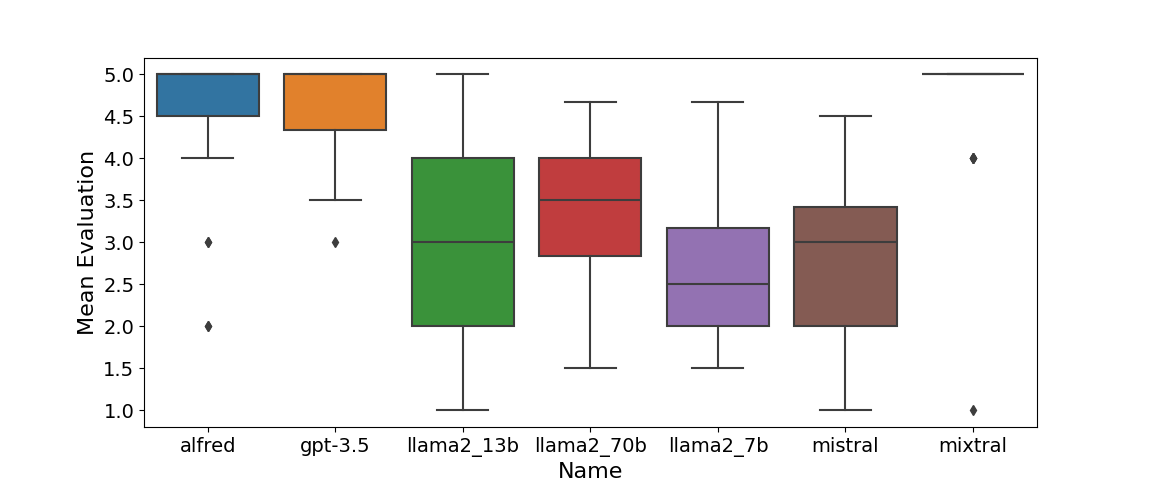
\includegraphics[width=0.9\textwidth]{figures/Figure_all.png}
	\caption{User-experience evaluation in the range [1-5] provided by domain experts for 210 responses, equally distributed, generated by the seven models.}
	\label{fig:eval-med}
\end{figure}

%% tre step

% 1) capacità di distinguere tra inserimento / richiesta dati e domande di qualunque altro tipo 

% 2) qualità della semantica della risposta nel dominio specifico rispetto a score allo stato dell'arte

% 3) do all'esperto le risposte a ciascun prompt e gli chiedo di dirmi qual è meglio

%cose da fare:
%- riesce a capire che le cose vanno trattate in modo diverso?--> fornire sul test set la risposta di classificazione nei contesti ipotizzati che dà modulo .Net allenato

%- fornire la risposta "definitva" del chatbot a tutte le domande del file di training-- funzione che chiama SU inserimento-- richiesta: facci-- umore+ generale: risposta precisa

%risposta completa

%%%%
%%%%
\section{Discussion}\label{sec:conc}

In this paper, we are taking concrete steps to explore the opportunities and limitations of LLM-based chatbot in medicine, 
in particular in the context of chronic disease self-management.
%
The peculiar characteristics of the context, force to deal with a set of issues that impose caution once delegating NLP\&NLG to an LLM that directly interacts with a patient, without the mediation of an expert. 
%
Particular attention should be given to the reliability and accuracy of the LLM's answers and to sensitive data protection.
%
Accordingly, specific solutions must be envisioned.

In this paper, we devised and tested two alternative solutions. 
%
Exploiting a model of the GPT family seemed the most obvious choice, since they demonstrated the best performances in all the tasks, compared to the others pre-trained LLMs\footnote{\url{https://lmsys.org/blog/2023-06-22-leaderboard/}}.
%
Properly prompted, it can be easily led to providing the minimum set of safe responses % valla a dimostrare però sta roba
to the patient, to avoid the disclosure of possible misinformation, still resulting empathetic, reassuring, and reliable.
%
However, some considerations come: 
\begin{enumerate}
    \item The risk of disclosing sensitive data still remains if the first filtering module fails;
    \item The call of a GPT-based model comes with the payment of a subscription;
    \item The free plan is limited in the number of overall tokens exchanged, in the number of requests/per minute and in the number of interactions/per day. As such, the solution does not scale with the number of users;   
    \item The dependence from third party services is a risk to be considered.
\end{enumerate}
%
\noindent The adoption of open models locally deployed resolves all these issues but results in a significant loss of response quality, as demonstrated in~
\Cref{fig:cm1,fig:cm2} Table~\ref{categorization:results} and Table~\ref{tab:req}. 
%
The ability of open models to correctly classify questions and properly extract parameters is strongly compromised in the solution that leverages open models, possibly requiring a fine-tuning to addressing these specific tasks.
%
However, Figure~\ref{fig:eval-med} brings forth a new perspective, where Alfred and Mixtral emerge as two open models whose responses to general questions are highly endorsed by domain experts. 
%
The paper findings thus highlight the delicate balance between privacy and improved patient interactions, essential for secure and informed healthcare communication, but at the same time foster new open models that warrant dedicated attention in future research aimed at enhancing their efficacy, particularly in areas where GPT-3.5 Turbo demonstrated superior performance in this study.

Accordingly, further investigations can consider a fine-tuning phase for each distinct task (i.e., sentence categorisation and general response), thereby enhancing the model's performance capabilities. 
%
This approach also offers a potential solution to language inconsistencies we encountered in Open-LLMs responses.
%
Furthermore, RAG can be considered to leverage the dataset that we collected for our comparison/training of ML.NET~2.0 framework, enabling the model to generate responses more in line with pre-existing outputs. Additionally, advanced prompt engineering strategies, such as the ``chain of thoughts''~\cite{wei2022chain} technique, could significantly improve the model's response accuracy. 
%
Lastly, exploiting larger models, such as Falcon 180b\footnote{\url{https://huggingface.co/tiiuae/falcon-180B}}, may provide enhancements similar to those observed in GPT-3.5 Turbo, presenting a promising direction for future research, even though the findings of this study underscore that model size alone does not guarantee enhanced performance.

\section*{Acknowledgements}

\paragraph{Statements of ethical approval}
This study has been conducted involving no patient, no volunteer, and no animal.
%
No personal or sensitive data has been exploited.

\paragraph{Fundings}

The authors declare that there was no financial support for this work.

\paragraph{Declaration of Competing Interest}
%
The authors declare that they have no known competing financial interests or personal relationships that could have appeared to influence the work reported in this paper.

\paragraph{Declaration of generative AI in scientific writing}
%
During the preparation of this work, the authors used GitHub’s Copilot in order to speed-up their writing.
%
After using this tool, the authors reviewed and edited the content as needed and take full responsibility for the content of the publication.

%\gamm{CRediT authorship contribution statement}


%% If you have bibdatabase file and want bibtex to generate the
%% bibitems, please use
%%
\bibliographystyle{elsarticle-num} 
\bibliography{biblio}

%% else use the following coding to input the bibitems directly in the
%% TeX file.

% \begin{thebibliography}{00}

% %% \bibitem{label}
% %% Text of bibliographic item

% \bibitem{}

% \end{thebibliography}
\end{document}
\endinput
%%
%% End of file `elsarticle-template-num.tex'.
